\hypertarget{logfile_8c}{
\section{logfile.c File Reference}
\label{logfile_8c}\index{logfile.c@{logfile.c}}
}
{\tt \#include $<$stdio.h$>$}\par
{\tt \#include $<$stdlib.h$>$}\par
{\tt \#include $<$time.h$>$}\par
{\tt \#include \char`\"{}logfile.h\char`\"{}}\par


Include dependency graph for logfile.c:\nopagebreak
\begin{figure}[H]
\begin{center}
\leavevmode
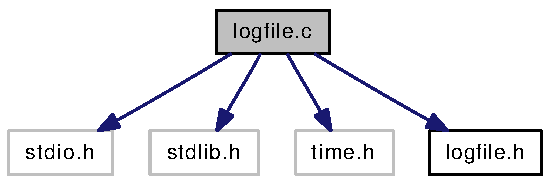
\includegraphics[width=150pt]{logfile_8c__incl}
\end{center}
\end{figure}
\subsection*{Functions}
\begin{CompactItemize}
\item 
char $\ast$ \hyperlink{logfile_8c_68a0e9d22417dfcf9c0be64261352e64}{asctime} (const struct tm $\ast$timeptr)
\item 
int \hyperlink{logfile_8c_f71f5daf2025b4e30a18ccedf7c34863}{write\_\-logentry} (char $\ast$msg, char $\ast$component, int flag)
\end{CompactItemize}


\subsection{Function Documentation}
\hypertarget{logfile_8c_68a0e9d22417dfcf9c0be64261352e64}{
\index{logfile.c@{logfile.c}!asctime@{asctime}}
\index{asctime@{asctime}!logfile.c@{logfile.c}}
\subsubsection{\setlength{\rightskip}{0pt plus 5cm}char$\ast$ asctime (const struct tm $\ast$ {\em timeptr})}}
\label{logfile_8c_68a0e9d22417dfcf9c0be64261352e64}


Compounds a humand readable date and time string.

\begin{Desc}
\item[Parameters:]
\begin{description}
\item[{\em timeptr}]A pointer to the actual time.\end{description}
\end{Desc}
\begin{Desc}
\item[Returns:]The date and time as a string. \end{Desc}


Definition at line 33 of file logfile.c.

Referenced by write\_\-logentry().

Here is the caller graph for this function:\nopagebreak
\begin{figure}[H]
\begin{center}
\leavevmode
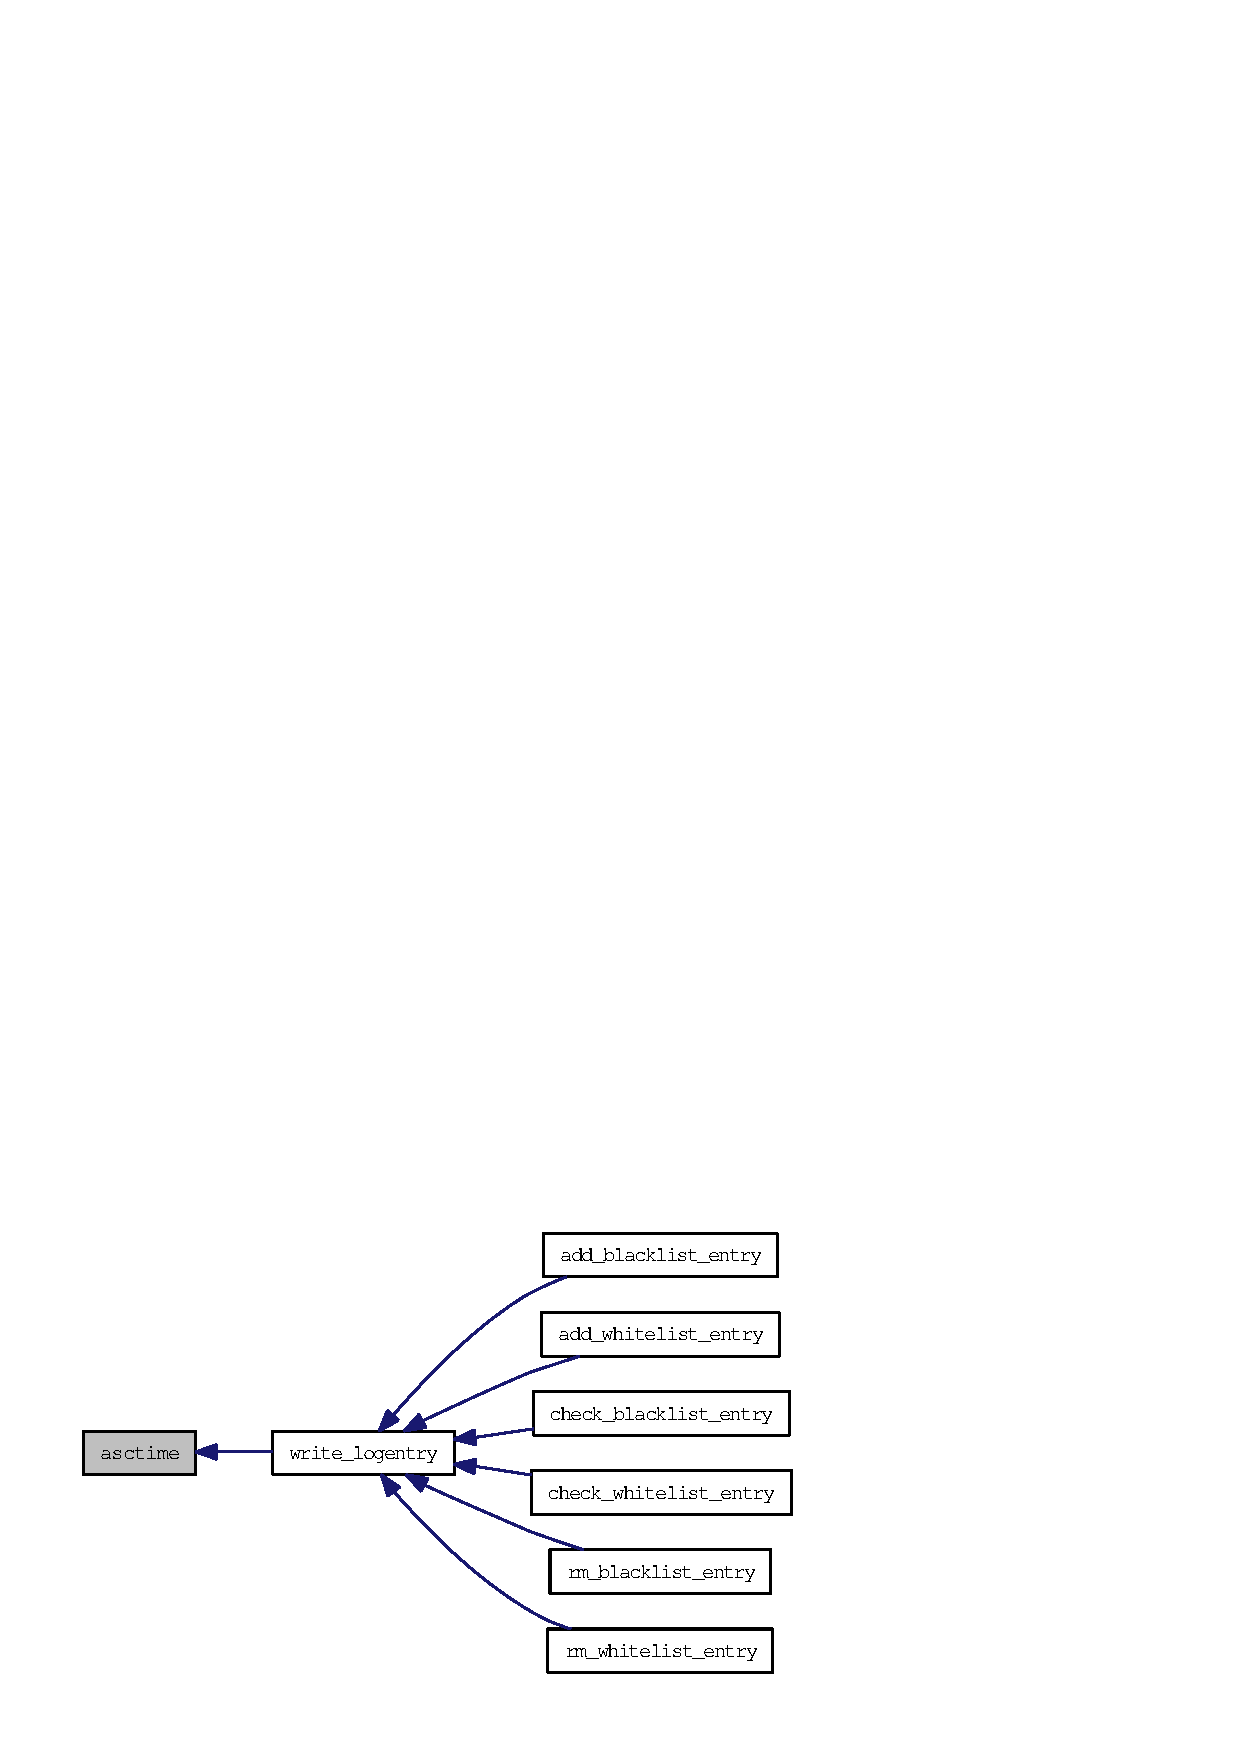
\includegraphics[width=109pt]{logfile_8c_68a0e9d22417dfcf9c0be64261352e64_icgraph}
\end{center}
\end{figure}
\hypertarget{logfile_8c_f71f5daf2025b4e30a18ccedf7c34863}{
\index{logfile.c@{logfile.c}!write\_\-logentry@{write\_\-logentry}}
\index{write\_\-logentry@{write\_\-logentry}!logfile.c@{logfile.c}}
\subsubsection{\setlength{\rightskip}{0pt plus 5cm}int write\_\-logentry (char $\ast$ {\em msg}, char $\ast$ {\em component}, int {\em flag})}}
\label{logfile_8c_f71f5daf2025b4e30a18ccedf7c34863}


Writes a logfile enty.

\begin{Desc}
\item[Parameters:]
\begin{description}
\item[{\em msg}]The message which should be written in the logfile. \item[{\em component}]The program which calls the write\_\-logentry function, for example \char`\"{}phonefirewall\char`\"{} \item[{\em flag}]What message should be written. Use the defined flags.\end{description}
\end{Desc}
\begin{Desc}
\item[Returns:]-1 if something fails, otherwise 0 \end{Desc}


Definition at line 58 of file logfile.c.

References asctime(), ERR\_\-FLAG, INFO\_\-FLAG, LOGFILE, MAX\_\-ENTRY\_\-LENGTH, UNKNOWN, and WARN\_\-FLAG.

Here is the call graph for this function:\nopagebreak
\begin{figure}[H]
\begin{center}
\leavevmode
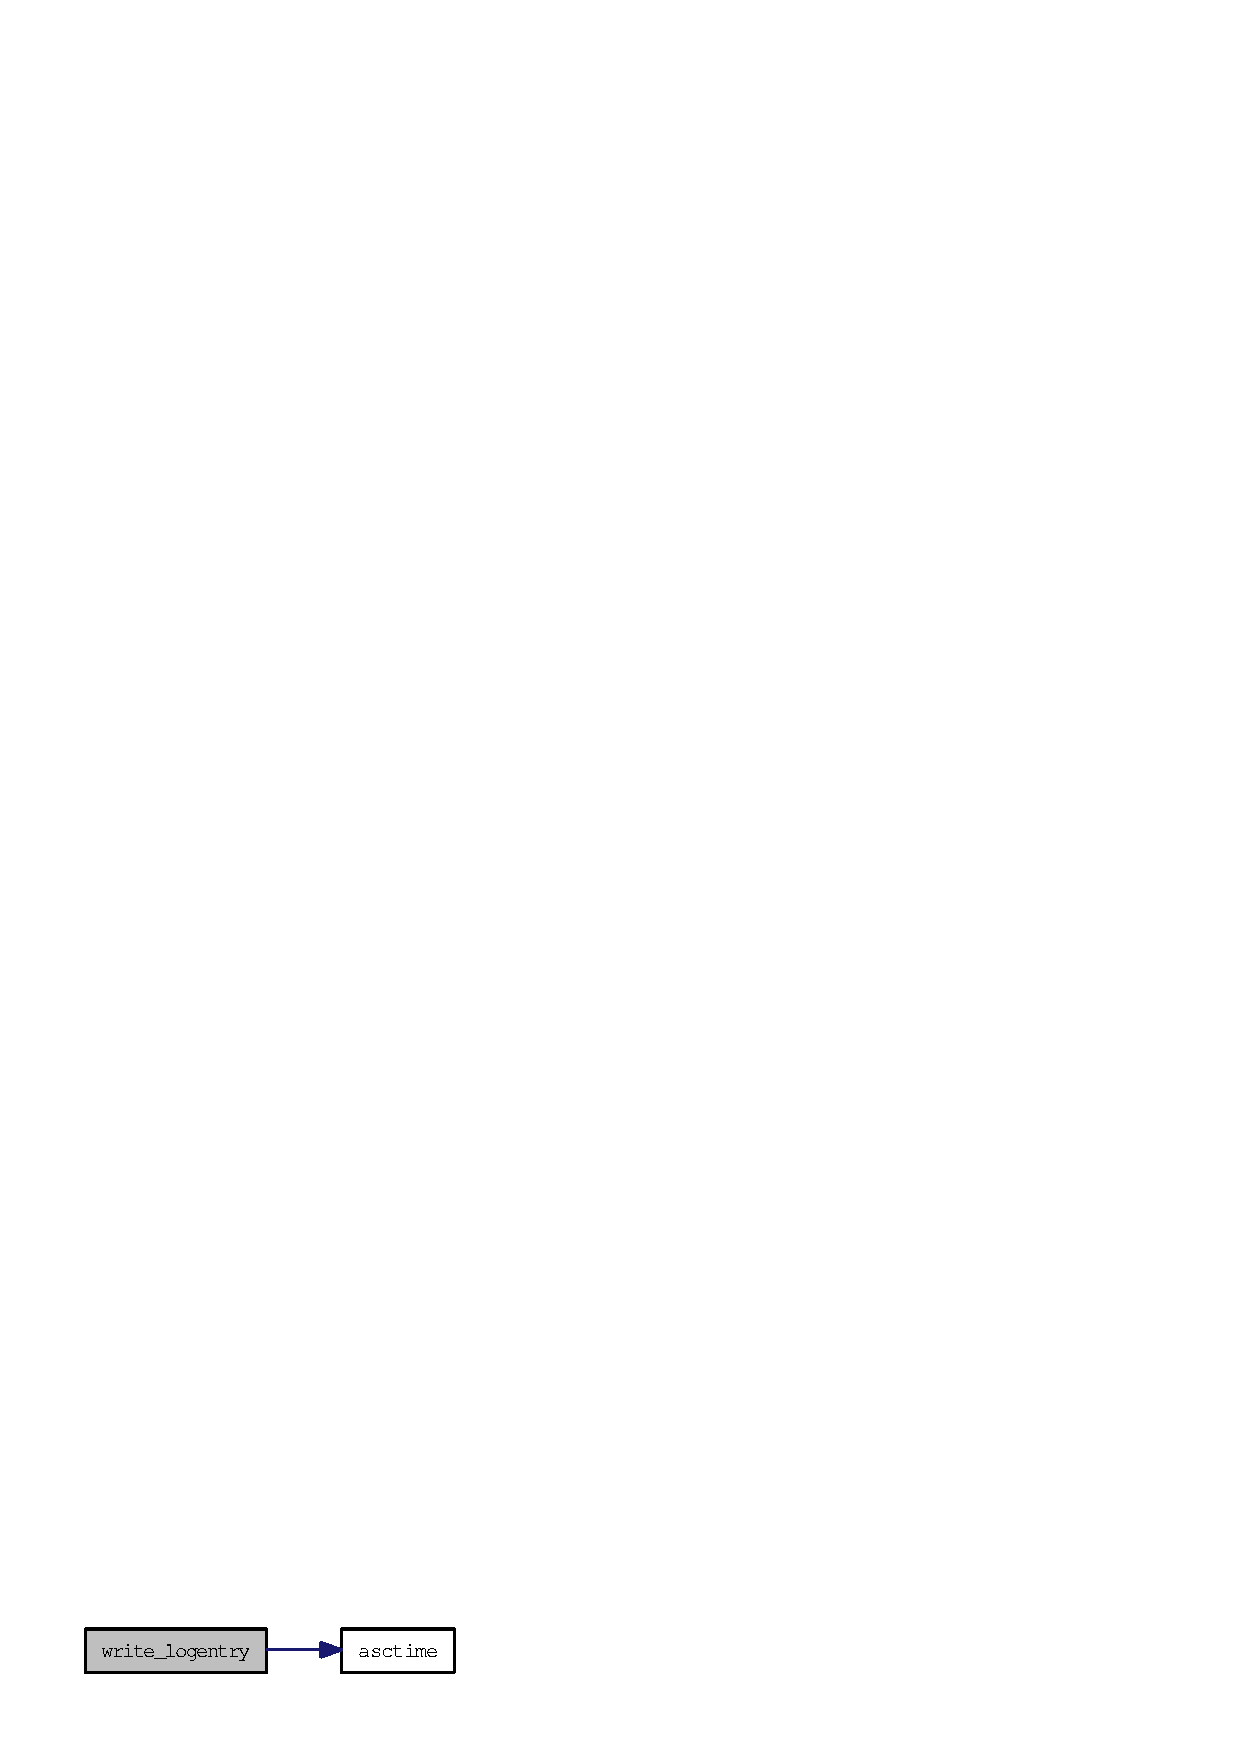
\includegraphics[width=111pt]{logfile_8c_f71f5daf2025b4e30a18ccedf7c34863_cgraph}
\end{center}
\end{figure}
